\documentclass[twoside,numberorder]{csbachelor}

%==============================================================
%==============================================================

\usepackage{url}
\usepackage{subfigure}

% 张海:其他引用
\usepackage[hidelinks]{hyperref}
\setlength{\LTpre}{1em}
\setlength{\LTpost}{1em}

\usepackage{tikz}
\usetikzlibrary{arrows,backgrounds,fit,shapes}
\tikzstyle{layer} = [draw, dashed]
\tikzstyle{block} = [draw, rectangle, minimum height=2em]
\tikzset{>=latex}

% 一些全局工具的定义
\DeclareMathOperator*{\argmin}{arg\,min}
\DeclareMathOperator*{\argmax}{arg\,max}

%==============================================================
%==============================================================

\begin{document}

%==============================================================
%==============================================================

  % 论文题目:{中文}{英文}
  \zjutitle{结合标签主题的跨域协同过滤算法}
           {Cross-domain Collaborative Filtering with Tag Topics}
  % 作者:{中文姓名}{英文}{学号}
  \zjuauthor{杨煜溟}{Yuming Yang}{3130000328}
  % 指导教师:{导师中文名}{导师英文名}
  \zjumentor{郑小林}{Xiaolin Zheng}
  % 个人信息:{年级}{专业名称}
  \zjuinfo{2013级}{计算机科学与技术}{Computer Science and Technology}
  % 学院信息:{学院中文}{学院英文}
  \zjucollege{计算机科学与技术学院}{College of Computer Science and Technology}
  % 日期:{提交日期}{Submitted Date}
  \zjudate{2017 年 6 月 5 日}{June 5, 2017}

%==============================================================

  {
    \pagestyle{empty}

    % {
  \setlength{\parindent}{0em}

  {
    \linespread{1}

    \vspace*{-1em}

    \begin{center}
      
\includegraphics[width=108mm]{data/cover-zh/xiaoming}
    \end{center}

    \vspace{-1.5em}

    {
      \songti\erhao\bfseries
      \centering
      本~~科~~生~~毕~~业~~论~~文 \par
    }

    \vspace{1em}

    \begin{center}
      
\includegraphics[width=35mm]{data/cover-zh/xiaobiao}
    \end{center}
  }

  \vspace{9em}

  {
    \linespread{1.6}
    \songti\sanhao\bfseries
    \centering
    \newlength{\titlelength}
    \setlength{\titlelength}{22em}
    题目 \; \underline{\makebox[\titlelength]{\zjutitlec}} \\
    姓名 \; \underline{\makebox[\titlelength]{\zjuauthornamec}} \\
    学号 \; \underline{\makebox[\titlelength]{\zjuauthorid}} \\
    指导教师 \; \underline{\makebox[\titlelength - 2em]{\zjumentorc}} \\
    年级与专业 \; \underline{\makebox[\titlelength - 3em]{\zjugrade \; \zjumajorc}} \\
    学院 \; \underline{\makebox[\titlelength]{\zjucollegec}} \\
    提交日期 \; \underline{\makebox[\titlelength - 2em]{\zjudatec}} \par
  }
}

    % {
  \setlength{\parindent}{0em}
  \linespread{1}

  \vspace*{-2.3em}

  {
    \songti\xiaoer
    \centering
    A Thesis Submitted to Zhejiang University \\
    for the Degree of Bachelor of Engineering \par
  }

  \vspace{3.6em}

  \begin{center}
    
\includegraphics[width=29.5mm]{data/cover-en/xiaobiao}
  \end{center}

  \vspace{3em}

  {
    \songti\xiaoer
    \centering
    TITLE \; \underline{\makebox[17em]{\zjutitlee}} \par
  }

  \vspace{1.1em}

  {
    \linespread{2}
    \begin{center}
    \sanhao
    \newlength{\majorlength}
    \setlength{\majorlength}{16em}
    \begin{tabular}{l l}
      Author & \underline{\makebox[\majorlength]{\zjuauthornamee}} \\
      Student ID & \underline{\makebox[\majorlength]{\zjuauthorid}} \\
      Supervisor & \underline{\makebox[\majorlength]{\zjumentore}} \\
      Major & \underline{\makebox[\majorlength]{\zjumajore}} \\
      College & \hspace{-3em}\underline{\makebox[\majorlength + 3em]{\zjucollegee}} \\
      Submitted Date & \underline{\makebox[\majorlength]{\zjudatee}} \\
    \end{tabular} \par
    \end{center}
  }
}


    % {
  \setlength{\parindent}{0em}
  \linespread{1}

  \vspace*{0.6em}

  {
    \centering
    \songti\xiaoer
    浙江大学本科生毕业论文(设计)独创性声明 \par
  }

  \vspace{3.1em}

  {
    \setlength{\parindent}{2em}
    \linespread{1.6}
    \songti\xiaosi
    本人声明所呈交的毕业论文(设计)是本人在导师指导下进行的研究工作及取得的研究成果。除了文中特别加以标注和致谢的地方外,文中不包含其他人已经发表或撰写过的研究成果,也不包含为获得 \underline{\kaiti\sihao\bfseries \makebox[5em]{浙江大学}} 或其他教育机构的学位或证书而使用过的材料。与我一同工作的同志对本研究所做的任何贡献均已在文中作了明确的说明并表示谢意。 \par
  }

  \vspace{2.9em}

  {
    \songti\xiaosi
    \begin{tabular}{@{} p{0.5\linewidth} p{0.5\linewidth} @{}}
    作者签名: & 日期: \hspace{4em} 年 \hspace{2em} 月 \hspace{2em} 日 \\
    \end{tabular} \par
  }

  \vspace{4.85em}

  {
    \centering
    \songti\xiaoer
    毕业论文(设计)版权使用授权书 \par
  }

  \vspace{2.2em}

  {
    \setlength{\parindent}{2em}
    \linespread{1.6}
    \songti\xiaosi
    本文作者完全了解 \underline{\kaiti\sihao\bfseries \makebox[5em]{浙江大学}} 有权保留并向国家有关部门或机构送交本文的复印件和磁盘,允许本文被查阅和借阅。本人授权 \underline{\kaiti\sihao\bfseries \makebox[5em]{浙江大学}} 可以将毕业论文(设计)的全部或部分内容编入有关数据库进行检索和传播,可以采用影印、缩印或扫描等复制手段保存、汇编毕业论文(设计)。

    (保密的毕业论文(设计)在解密后适用本授权书) \par
  }

  \vspace{2.9em}

  {
    \songti\xiaosi
    \begin{tabular}{@{} p{0.5\linewidth} p{0.5\linewidth} @{}}
    作者签名: & 导师签名: \\
     & \\
     & \\
    日期: \hspace{4em} 年 \hspace{2em} 月 \hspace{2em} 日 & 日期: \hspace{4em} 年 \hspace{2em} 月 \hspace{2em} 日 \\
    \end{tabular} \par
  }
}

    \cleardoublepage
  }

  {
    \frontmatter

    \pagestyle{frontmatter}
    \makeatletter
      \let\ps@plain\ps@frontmatter
    \makeatother

    \chapter{摘要}

标签系统的普及为提升推荐算法的性能提供了可行的途径,用户赋予物品的标签中蕴涵了丰富的信息,利用这些信息可以缓解数据稀疏性问题。现有的方法大都在单一域上对评分和标签进行建模,而没有利用标签的特性将不同域连接起来。

本文中,我们提出了一个基于评分和标签的跨域协同过滤模型,首先利用主题建模挖掘物品标签的语义信息,并将标签主题结合到传统的矩阵分解模型中,之后将标签作为连接不同域的桥梁,利用辅助域的信息帮助目标域的推荐任务。

在两个真实数据集上的实验表明,我们提出的模型有效地缓解了数据稀疏性问题,相较于传统的矩阵分解方法和结合标签的协同过滤方法具有明显的优势。

{
    \vspace{1em}
    \setlength{\parindent}{0em}
    \textbf{关键词} \; 推荐系统 \; 协同过滤 \; 跨域\; 主题模型 \; 标签 \par
}

    \chapter{Abstract}

The popularity of tagging systems provides effective ways to improve the performance of recommendation algorithms. The tags assigned by users to items contain rich information, which can be utilized to alleviate data sparsity limitations. Most existing approaches focus modeling tags and ratings on single domain, they overlook an important property that tags link different domains as a bridge. 

In this paper, we propose a novel tag and rating based cross-domain collaborative filtering model, which first uses topic modeling to mine the semantic information of tags labelled for items, and then incorporates the semantic information into matrix factorization to factorize rating information. At last, we investigate how to utilize the bridging feature of tags between totally different domains to improve the rating prediction task in target domain.

Experiments conducted on two popular real-world datasets demonstrate that our proposed model significantly outperforms the conventional CF approach, the state-of-the-art tag and rating based CF approach in terms of both RMSE and MAE, and it is an effective approach to the data sparsity and the cold-start problem.

{
    \vspace{1em}
    \setlength{\parindent}{0em}
    \textbf{Keywords} \; Recommendation system \; Collaborative filtering \; Cross-domain \; Topic model \; Tags \par
}


    \tableofcontents
    \newpage
    \thispagestyle{empty}
  }


  {
    \mainmatter

    \pagestyle{mainmatter}
    \makeatletter
      \let\ps@plain\ps@mainmatter
    \makeatother

    %!TEX root = ../main.tex
\chapter{绪论}

\section{课题背景}

随着信息技术和互联网的发展,人们逐渐从信息匮乏的时代走入了信息过载的时代,海量信息的复杂性和不均匀性使得信息获取变得困难而耗时,无论信息消费者还是信息生产者都遇到了很大的挑战。关于信息过载的问题,代表性的解决方案是分类目录和搜索引擎\cite{项亮2012推荐系统实践},分类目录只能覆盖少量内容而越来越不能满足用户的需求,搜索引擎可以让用户通过搜索关键词找到自己需要的信息,但是,搜索引擎需要用户主动对需求提供描述,当用户无法找到准确描述自己需求的关键词时,搜索引擎就无能为力了。

个性化推荐系统根据用户过往的行为,分析用户的兴趣模式,自动为用户过滤掉低相关的内容,呈现符合用户品味的个性化的产品建议,大大降低了用户检索信息的成本。与搜索引擎不同,推荐系统不需要用户提供明确的需求,从某种意义上来说,推荐系统和搜索引擎是两个互补的技术,推荐系统满足了用户有明确目的时的主动查找需求,而推荐系统能够在没有明确目的时帮助用户发现感兴趣的内容。

应用个性化推荐技术需要两个条件,第一个是存在信息过载的情况,第二个是用户在大部分时候没有明确的需求。越来越多的网站成功地引入了推荐系统,广泛利用推荐系统的领域包括电子商务、电影和视频、音乐、社交网络、基于位置的服务、个性化广告等。

推荐系统可关联到很多相关研究领域,例如用户建模、机器学习和信息检索等 \cite{fernandez2012cross} 。由于其与日俱增的重要性,它在 20 世纪 90 年代发展成一个独立的研究领域 \cite{肖力涛2016基于隐式因子和隐式主题的跨域推荐算法研究}。在推荐的过程中,推荐的准确性,以及推荐算法的效率等问题就是推荐算法研究的着重点。

推荐系统依赖于不同类型的用户行为数据,最理想的是高质量的显式反馈行为,即用户对物品兴趣的明确输入,主要的方式就是评分。通常,显式反馈产生稀疏的偏好度矩阵。与之相对应的是隐式反馈行为,即那些不能明确反应用户喜好的行为,例如购买商品、浏览页面、评论或甚至鼠标移动。相比显式反馈,隐式反馈虽然不明确,但数据量更大,因此可以利用隐式反馈缓解数据稀疏性问题。

推荐系统根据用户的历史行为预测未来的行为和兴趣,因此大量的用户数据是实现推荐系统的前提。用户物品的偏好度矩阵通常是非常稀疏的,因为单个用户浏览或使用过的物品只是很小的一部分,这样的稀疏矩阵导致潜在的关联度降低,影响推荐算法对用户兴趣的建模。另外,对于系统中加入的新用户或新物品,因为没有他们的历史数据,就无法为其关联其它用户或物品,这就产生了冷启动问题。如何克服冷启动和数据稀疏性问题是目前研究面临的主要挑战。


\section{本文的主要工作}
为了缓解上面提到的冷启动问题和数据稀疏性问题,本文提出了一种结合标签主题的跨域推荐算法(Cross-domain Collaborative Filtering with Tag Topics)。

目前,一个研究的趋势是在协同过滤中混合主题模型来处理文本内容信息,例如,Wang 和 Blei 提出了一个协同主题回归(CTR)\cite{Wang2011Collaborative}模型用于学术文章的推荐,在冷启动问题上取得了良好的效果。

跨域推荐尝试利用辅助域中的信息来协助目标域上的推荐,现有的跨域方法大都要求不同域之间存在共享用户,我们希望找到在没有共享用户的情况下关联多个域的方法,利用跨域推荐提高推荐系统的效果。

在本文的研究中,我们依赖于不同域中的重叠的标签词汇,将标签作为连接不同域的桥梁,例如,标签“romantic”可以用于描述一个电影,也可以是一首歌曲或是一处风景。因此,目标域可以学习到辅助域中的某个标签对评分的影响,即,如果在辅助域中的某个标签存在时,关联的评分通常较高,则可以将这种依赖关系从辅助域传递到目标域。

本文提出的模型在传统的矩阵分解模型的基础上,引入标签这种隐式反馈信息,使用主题建模采集标签中的语义信息,提高单一域上的推荐效果。之后,我们将跨域推荐的思想结合进来,利用辅助域中丰富的标签信息,使得模型在较为稀疏的数据集上具有良好的表现。

为了评估我们提出的模型的效果,我们使用两个真实的数据集进行了一系列实验,并将结果与现有的推荐算法进行了比较,说明结合标签信息对于提升推荐效果具有帮助。


\section{本文结构安排}
本文分为五个章节:

第一章主要介绍了本文的课题背景,并针对传统模型的问题进行了分析,提出本文的主要内容和研究思路。

第二章是相关技术综述,首先在整体上介绍了推荐系统的研究现状,之后详细介绍了基于协同过滤的推荐算法、LDA 主题模型以及跨域推荐的思想。

第三章提出了本文的结合标签主题的跨域推荐算法,并说明了模型参数的学习方法。

第四章从数据集的预处理、评价标准以及参数的选取等方面对实验进行了介绍,将提出的模型与现有的算法进行比较,论证本文模型的有效性。

第五章总结了本文的主要工作,并提出未来可以改进的方向。




    \cleardoublepage
    %!TEX root = ../main.tex
\chapter{相关工作综述}

\section{推荐系统的研究现状}

推荐算法的本质是通过一定方式将用户和物品联系起来,常用的方式有利用好友关系、用户的历史兴趣以及用户的注册信息等\cite{项亮2012推荐系统实践}。概括地说,推荐系统主要基于两种不同的方法或它们的组合:基于内容的方法和基于协同过滤的方法。

基于内容的推荐方法为用户和物品赋予简要的描述,以表示各自独特的性质,例如,电影的描述可以包括其类型、导演、票房等方面,用户的描述可以是个人资料或从已评分物品中识别出的共同特征,这样可以利用描述为用户匹配合适的物品。这种方式的好处很明显,透明度高,推荐方式直接,而且当有新物品出现时,利用物品的描述即可进行推荐。然而缺点也较为明显,基于内容的策略需要收集额外的信息,而这些信息可能并不容易得到,同时隐私问题也可能阻碍用户提供个人信息\cite{Koren2009Matrix}。

另一种策略,不像内容过滤那样需要明确的描述信息,而是围绕用户物品的评分矩阵,分析用户之间的关系和物品之间的相互依赖性,以获得新的用户和物品的关联,这种方法被称为协同过滤(Collaborative Filtering)\cite{Goldberg1992Using}。协同过滤算法是目前推荐系统研究的热点之一,大多数推荐算法都是在此基础上改进而来。传统的协同过滤仅利用评分信息进行推荐\cite{shi2014collaborative},主要分为两种类型,基于近邻的方法\cite{Desrosiers2011A,Sarwar2001Item,Deshpande2004Item}和基于潜在特征模型的方法\cite{xu2015ice}。前者直接利用存储在系统中的用户项目评分进行预测,因此又被称为基于存储的协同过滤。后者尝试从偏好度矩阵中推断出用户和物品的低维的特征向量映射,基于模型的方法具有良好的可扩展性和预测精确性而变得流行。传统的协同过滤克服了基于内容的一些限制,它比内容过滤的技术更加精确,但是却面临数据稀疏性和冷启动问题。因此,一些借助文本内容的信息的混合模型被提出来。

在协同过滤模型中引入内容信息是当今的研究热点之一,主题建模算法\cite{blei2009topic}用于从大量文档中发掘潜在的主题,主题模型提供了文档的低维表示\cite{Chang2009Reading},代表性的主题模型有隐式狄利克雷分布(LDA)\cite{Blei2003Latent},该模型的假设是文章与词之间是通过主题联系的。协同主题回归模型(CTR)\cite{Wang2011Collaborative}结合了基于潜在因素模型 \cite{Agarwal2009Regression,Salakhutdinov2007Probabilistic} 的协同过滤的思想和基于概率主题模型的内容分析\cite{Blei2003Latent,Chang2009Reading,Agarwal2010fLDA},使得系统在冷启动问题上表现良好。CTR-SMF \cite{purushotham2012collaborative} 以及 CTR-SMF2 \cite{chen2014context} 模型将社交信任矩阵引入 CTR 模型,以进一步提高推荐性能。


跨域推荐是一个新兴的研究课题,它旨在利用辅助域中的用户反馈来缓解目标域上的稀疏性问题\cite{hu2013personalized}。虽然跨域推荐的效果可能不如在单一域上的推荐准确,但跨域推荐将更加多样化,这可能对提高用户的满意度和参与度有好处。跨域推荐的关键挑战是在不同域的项目和用户之间发现有用的联系,通常所考虑的域之间看上去是不相关的,例如,音乐与感兴趣的地方,因此很难找到它们之间的关联\cite{shi2011tags},对于如何发掘不同域的信息产生了多种观点,例如,
Li 等人提出了基于迁移学习的方法\cite{li2009can},该方法将辅助域的稠密评分矩阵进行共现聚类并发掘每个类的评分模式,利用评分模式建立不同域之间的关联,在另外的工作中\cite{li2009transfer},假设用户和物品属于某个类服从概率分布,利用概率模型扩展了该方法。而基于连接的跨域模型利用标签或评论信息可以用于发掘不同域的用户或物品的兴趣\cite{kaminskas2011location,Enrich2013Cold,Xin2015Cross},因为不同域中用户产生的内容通常会具有关联。Zhuang \cite{zhuang2010cross} 等利用香农熵和逻辑回归进行一致性计算,从而建立不同域之间的关联。Cao \cite{cao2010transfer} 等提出一种概率贝叶斯框架解决了连接预测的问题,即预测在用户和物品之间的潜在连接。


标签系统的普及促进了推荐系统的发展,标签中蕴含着丰富的有价值的信息,用户用标签来描述对物品的看法,当一个用户为一些物品赋予了标签,那这些标签就反映了用户对物品的偏好\cite{chen2016capturing},如何利用标签数据提高个性化推荐的质量是推荐系统的重要课题\cite{项亮2012推荐系统实践}。目前,标签系统中主要有两种类型的协同过滤,标签推荐\cite{wang2013collaborative,fang2015personalized}的目的是为物品匹配合适的标签,另一种是基于标签的物品推荐\cite{zhou2010userrec,xu2011semrec},它旨在利用标签和评分等信息为目标用户推荐用户或物品。

\section{基于协同过滤的推荐系统}
协同过滤(Collaborative Filtering)是推荐系统中应用最早和最为成功的策略之一,这个术语最早由 David Goldberg 等人于 1992 年创造 ,用于描述一个实验性的邮件过滤系统 Tapestry \cite{Goldberg1992Using}。协同过滤克服了基于内容过滤的一些限制,它不使用内容信息,而是通过分析系统中其他用户和物品的评分信息,以获得新的用户和物品的关联。

随着互联网的不断发展,尤其是电子商务的出现,推荐算法随之快速发展,协同过滤在研究领域和实践中都去得了巨大成功,目前大部分推荐算法都是基于协同过滤算法改进而来,协同过滤的两个主要领域是基于近邻的方法和潜在因素模型。

\subsection{基于近邻的协同过滤}
最常见的协同过滤是基于近邻的方法,该方法的基本思想借鉴了人们生活中选择物品的方式,如果身边的朋友喜欢某件物品,那么自己就会有很大概率选择该物品。另外,如果用户喜欢某个物品,那么他很可能喜欢与该物品类似的物品。因此,该方法又分为基于用户的方法和基于物品的方法。

在基于近邻的协同过滤中,存储在系统中的用户项目评分直接用于预测新项目的评分,因此有被称为基于存储的协同过滤。该算法在用户评分矩阵并不稀疏的时候能够产生非常良好的效果,而且不需要训练,直接通过计算就可以给出推荐,但是当数据量非常庞大的时候,推荐过程伴随着大量的计算,这也从一定程度上阻碍该算法在线上系统当中的使用。

\subsubsection{基于用户的近邻推荐}
协同过滤最初的形式是以用户之间的关系为中心\cite{Desrosiers2011A},系统的实现分为两个阶段,首先在历史数据中发现那些具有相似品味的用户,然后利用邻居对物品 $i$ 的评分计算用户 $u$ 对一个新物品 $i$ 的评分 $r_{ui}$ 。假设我们计算得到了每个用户对 $u \neq v$ 之间的相似度 $w_{uv}$ ,与用户 $u$ 相似度最高的 $k$ 个用户的集合,称为 $u$ 的 $k$ 近邻($k$ -NN),该集合记为 $N(u)$。然而只有评价过物品 $i$ 的邻居才可以用来预测 $r_{ui}$ ,因此我们将这个邻居的集合记为  $N_i (u)$ ,可以用这些邻居对 $i$ 评分的平均值来估计  $r_{ui}$ :
\begin{equation}
\hat{r_{ui}} = \dfrac {1}  {| N_i (u) | }   \sum_{v \in  N_i (u)}{ r_{v,i} } .
\end{equation}

这个式子并没有考虑到邻居间可以具有不同相似度的问题,可以利用每一个邻居与 u 的相似度对评分加权平均。

\subsubsection{基于物品的协同过滤}
比较流行的是基于物品的方法\cite{Sarwar2001Item,linden2003amazon},基于用户的推荐依赖于“志同道合的用户”的观点,而基于物品的方法着重于相似物品的评分。为了使用相似性度量,首先确定 $u$ 选择过的与 $i$ 最相似的 $k$ 个物品,这 $k$ 个近邻的集合由 $N_u (i)$  表示,预测值 $r_{ui}$ 的计算方法是采用 $u$ 在集合 $N_u (i)$  中评分的加权平均:
\begin{equation}
\hat{r_{ui}} = \dfrac { \sum\limits_{j \in N_u (i)} w_{i,j} r_{u,j}}  {\sum\limits_{j \in N_u (i)} w_{i,j} } .
\end{equation}

\subsubsection{相似性权重计算}
构建基于近邻的推荐系统的最关键方面之一是相似性权重的计算,它对推荐系统的准确性和性能具有显著影响。相似性的计算基于这样的共识:相似的用户喜欢相似的物品,同时相似的物品被相似的用户喜欢。目前有多种方式用于相似性的计算,最常见的是将评分矩阵中的行列向量作为对应用户或物品的抽象,然后计算向量余弦夹角。实际上,当使用显式评分作为偏好度时,不同的用户往往会有差异,例如某些用户的评分普遍偏高,可以使用与评分平均值的偏移作为偏好度,因此,采用这种调整的余弦相似度,物品 $i$ 和 物品 $j$ 之间的相似度计算方法如下(以计算物品间相似性为例):
\begin{equation}
sim(i,j) = \dfrac{\sum\limits_{u \in U} (r_{u,i} - \bar{r_u})  (r_{u,j} - \bar{r_u})} {   \sqrt {\sum\limits_{u \in U}  {(r_{u,i} - \bar{r_u})}^2  }    \sqrt {\sum\limits_{u \in U}  {(r_{u,j} - \bar{r_u})}^2  }  } ,
\end{equation}
其中,$r_u$ 是用户 $u$ 评分的平均值。通常上不必考虑所有近邻,为相似度定义一个具体的最小阈值,或者将规模限制为一个固定值,而且只考虑 $k$ 个最近邻\cite{Jannach2010Recommender}。

\subsubsection{基于用户与物品方法对比}
应用基于近邻的协同过滤系统时,可以从以下几个方面考虑选择基于用户还是基于物品的方法\cite{Desrosiers2011A}:
\begin{enumerate}
	\item {准确性}:在电子商务系统中,用户的数量往往远大于商品的数量,数据的稀疏性会导致很难匹配到相似用户,因此推荐的精确性将收到严重影响,此时使用基于物品的方法会有更高的准确性。同样的,在用户数量少于物品的场景下,例如学术论文推荐系统,采用基于用户的方法会比较准确。

	\item {效率}:推荐算法的计算量和存储量也取决于用户和物品的比例,当用户量远超物品数量,计算用户之间的相似性会产生庞大的计算量,影响系统的可扩展性。因为用户只对少数物品评级,因此仅存储非零的或者前 $N$ 个相似性权重可以降低存储量和在线推荐的复杂度。

	\item {稳定性}:一般情况下系统中可用的物品与用户相比是更加静态的,因此物品相似性权重可以不用频繁地计算,这样,利用用户当前的数据可以进行实时的查询推荐,相比于基于用户的方法,系统具有更高的稳定性。

	\item {可辨识性}:面向物品的方法更适合解释推荐背后的原理,这是因为用户往往熟悉之前选择过的物品,而不知道那些所谓志同道合的用户。这样,可以向用户展示在当前预测中使用的邻居物品列表以及它们的相似性权重,通过修改列表或权重,用户可以交互的参与推荐过程。

\end{enumerate}


\subsection{基于潜在特征的协同过滤}
基于模型的方法不直接利用存储的评分进行预测,而是尝试从偏好度矩阵中推断出用户和物品的低维的特征向量映射,某种意义上,特征向量隐含了用户和物品在多个维度上的性质。在该模型中,用户对物品的预测偏好度是特征向量的线性结合。例如,每一个物品 $i$ 与向量 $q_i \in R^f$ 相关联,每一个用户 $u$ 与向量 $p_i \in R^f$ 相关联,它们的内积 $q_i^Tp_u$ 表现了用户 $u$ 对物品 $i$ 在 $f$ 个特征上的总体偏好度。 因此评分的估计由如下式子给出:
\begin{equation}
\hat{r_{ui}} = q_i^Tp_u.
\end{equation}
这种方法最主要的挑战是如何将每一个用户和物品映射到特征向量 $q_i, p_u \in R^f$ ,在完成了映射之后,推荐系统将很容易利用上面的公式预测用户对物品的评分。潜在特征向量映射的实现通常是基于矩阵分解的,奇异值分解(SVD)\cite{paterek2007improving}是一种最基本的矩阵分解算法,它的计算方式是使得到的矩阵与原始矩阵对应项的正则平方和误差最小:
\begin{equation}
\min_{q^*, p^*} {\sum\limits_{(u,i) \in \kappa} {{(r_{u,i}-q_i^Tp_u)}^2 + \lambda(||q_i||^2 + ||p_u||^2)} } ,
\end{equation}
这里,$\kappa$ 是训练集中所有已知评级的用户物品对 $(u,i)$ 的集合,系统通过拟合之前观测的样本来学习模型的参数,而我们的目标是预测未知的评分,所以应该通过正则化参数来避免过度拟合已知的项,常数 $\lambda$ 用于控制正则化的程度。

可以通过随机梯度下降算法(stochastic gradient descent)最小化上面的误差函数。首先通过求参数的偏导数找到函数的最速下降方向,然后不断迭代优化参数直至收敛。上面定义的函数里有两组参数 $p_{u}$ 和 $q_{i}$ ,对它们分别求偏导数,然后梯度相反的方向以 $\gamma$ 步长调整参数,可以得到如下的迭代公式:
\begin{equation}
\begin{aligned}
&q_i \leftarrow q_i + 𝛾 \cdot(e_{ui} \cdot p_u -\lambda \cdot q_i),\\
&p_u \leftarrow p_u + 𝛾 \cdot(e_{ui} \cdot q_i- \lambda \cdot p_u),
\end{aligned}
\end{equation}

样本数据中通常会存在用户和物品个体性的偏移,例如一些用户给分普遍偏高。因此,直接将 $q_i^Tp_u$ 视为最后的评分值是不明智的,可以为每个用户和物品设置偏移量,加入偏移后改写为如下形式:
\begin{equation}
\hat{r_{ui}} = \mu + b_i + b_u + q_i^Tp_u.
\end{equation}
其中,$\mu$ 是全部评分的平均值,参数 $b_i$ 和 $b_u$ 是在样本上用户 $u$ 和物品 $i$ 的偏移量。这样,观察到的评分被分为了四个组成部分:全局平均、用户偏移、物品偏移、用户物品匹配,这使得每一个部分可以单独解释其含义。



\section{概率主题模型}
主题建模算法用于从大量文档集合中发现一组主题,其中主题是关于词项的分布,主题模型提供了文档的低维表示\cite{Chang2009Reading},通常被用于语料库检索、文档分类和信息检索等任务。最常见的主题模型是隐式狄利克雷分布(LDA)\cite{Blei2003Latent},假设有 $K$ 个主题 $\beta_{1:k}$,每一个都是在固定词典上的分布。LDA 生成文档的大致流程如下:
对于语料库中的每一篇文档 $w_{jn}$ :
\begin{enumerate}
\item 从狄利克雷分布中选取主题分布 $\theta_j \sim Dirichlet(\alpha).$
\item 对于文档中的每一个词 $n$ :
	\begin{enumerate}
		\item 选取主题 $z_{jn} \sim Mult(\theta_j).$
		\item 选取单词 $w_{jn} \sim Mult(\beta_{z_{jn}}).$ 
	\end{enumerate}
\end{enumerate}
这个过程说明了文档中的每个词是如何从主题的集合中选取出来的:主题分布是文档特有的,但是主题的集合是整个语料库共享的。不像聚类模型那样每个文档只能属于一个类别,LDA 允许文档具有多个主题。
\begin{figure}[htbp]
\centering
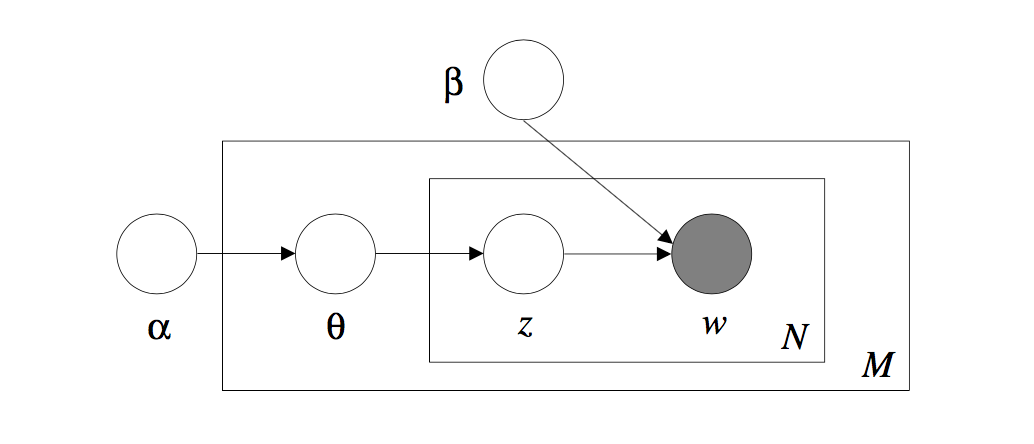
\includegraphics[width=0.7\linewidth]{images/lda.png}
\caption{LDA 的图模型。方框代表重复,外层的方框表示文档,而内层的方框表示文档中不断重复选择的主题和单词。}
\label{fig:fig1}
\end{figure}

LDA 属于非监督学习的范畴,给定一个文档语料库,我们可以使用变分 EM 算法来学习主题并根据它们给文档分配主题\cite{Blei2003Latent}。此外,给定一个新的文档,我们可以使用变分推理来确定其内容的主题。

矩阵分解的一个优点是它允许在特征向量中加入附加信息。Wang and Blei \cite{Wang2011Collaborative} 提出了协同主题回归模型(CTM)用于学术文章的推荐,该方法使用两种类型的数据:用户的收藏历史和文章的内容,结合了基于潜在因素模型 \cite{Agarwal2009Regression,Salakhutdinov2007Probabilistic} 的协同过滤的思想和基于概率主题模型的内容分析\cite{Blei2003Latent,Chang2009Reading}。模型很好的利用了内容信息,并将其结合到了传统的协同过滤算法中,使得系统在物品冷启动问题上表现良好。

\section{跨域推荐系统}
现有的推荐算法大多是仅针对属于单个域内的用户物品进行建模,因此是在单一域上的建模。事实上,用户在不同域中的偏好之间可能存在依赖性和相关性,例如,直观上来看,喜欢摇滚音乐的用户很可能喜欢科幻片,喜欢抒情音乐的用户或许喜欢爱情片。因此,在一个域中获得的用户兴趣特征可以在几个其他域中传递和利用,而不是独立地处理每种类型的项目。虽然跨域推荐的效果可能不如在单一域上的推荐准确,但跨域推荐将更加多样化,这可能对提高用户的满意度和参与度有好处 \cite{fernandez2012cross}。

Leizou \cite{Loizou2009How} 提出跨域推荐的三个主要研究趋势:
\begin{enumerate}
\item 通过集成和利用分布在不同系统中的显式用户偏好。
\item 通过记录用户的行为和反应来描述用户特征,并利用这些信息生成多个域上的推荐。
\item 通过组合来自不同域的推荐来生成单一域上的推荐。
\end{enumerate}

当两个域之间的用户和物品存在重叠时,我们可以直接将所有的信息看作属于一个共同的域,这样就可以利用传统的协同过滤进行跨域推荐。然而,当两个域没有重叠或重叠很小时,这种方法就会产生问题。为了解决上述不重叠的情况,我们必须找到某种方法,能够在域之间找到或建立某种类型的显式或隐式关系,其将被用作在推荐系统中连接不同域的桥梁\cite{fernandez2012cross}。

\subsection{基于迁移学习的模型}
迁移学习是机器学习领域的热门研究课题,基于迁移学习的跨域CF模型旨在通过对多个域的用户反馈建模来挖掘迁移模式,一种方法是在不同域中映射用户的特征向量,对于一个用户 $a$ ,假定他在目标域的特征向量是 $U_a$ ,辅助域中的为 $U'_a$ ,我们的目标是找到它们之间的映射函数,使得它们可以相互转换以提高两个域的效果。直观上,理想的情况是找到 $U_a$ 和 $U'_a$ 之间的可逆映射函数,但是有时候这种关系是非线性的,在这种情况下不能找到可逆函数 \cite{Xin2015Cross}。

在迁移学习的框架下,学习过程的每一次迭代,先利用随机梯度下降等算法更新单个域中的参数,然后利用域间的映射函数进行估计并得到误差,以最大后验概率的方式调整映射函数的参数。该方法的限制是需要依赖跨域共享的用户,即存在一些用户在多个域上都有行为数据。实际中,为了降低噪声干扰和复杂性,通常只利用那些在两个域都有密集活动的用户集合来训练模型。

\subsection{基于语义桥的跨域推荐}
基于连接的跨域协同过滤利用不同域间的具有相似内容的信息,将不同域间的物品连接起来。典型的方法是使用标签来桥接这些物品 \cite{Enrich2013Cold,chen2016capturing},因为不同域中使用的标签词汇之间的通常是重叠的\cite{项亮2012推荐系统实践},如果一个用户在辅助域中喜欢一个物品并赋予该物品某个标签,那么他也很可能喜欢目标域中具有相同标签的物品 \cite{Xin2015Cross}。例如,喜欢“romantic”电影的用户可能也喜欢“romantic”的书籍。

UserItemTags  \cite{shi2011tags}是一个结合标签的跨域推荐模型,它实现了在没有共享用户的情况下,利用辅助域信息缓解目标域的稀疏性问题。他们基于的假设是一个用户给一个物品的评分依赖于该用户赋予该物品的独特的标签,因此该模型在进行评分预测时,结合考虑目标用户赋予目标物品的标签。对于一个用户 $u$ ,一个物品 $i$ 和用户赋予物品的标签集合 $T_u(i)$ ,该算法依据如下规则预测评分:
\begin{equation}
\hat{r_{ui}} = p_u^T \cdot (q_i + \frac{1}{|T_u(i)|}  \sum\limits_{t  \in T_u(i)} {y_t}  ),
\end{equation}
其中,$p_u$,$q_i$ 和 $y_t$ 分别是用户 $u$、物品 $i$ 和标签 $t$ 的潜在特征向量。该模型参数的学习方法与 SVD 相同,采用随机梯度下降最小化正则平方误差,差别在于该模型同时遍历目标域和辅助域的评分和标签。

这个模型的主要限制是必须借助目标用户对目标物品的标签集合 $T_u(i)​$ ,而对于未被目标用户赋予标签的物品,则无法进行评分预测。本文在该模型的基础上进行改进,解决了上述限制,并挖掘了标签的主题,引入了语义信息,提高了推荐的效果。

\section{本章小结}

本章介绍了推荐系统目前的研究现状,从基本的协同过滤方法开始讨论,引出推荐系统中冷启动和稀疏性等关键的问题,并阐述了主题模型的思想,以及当今比较热门的跨域推荐的相关概念,内容基本涵盖了本文模型涉及到的相关技术。

本文的目标是将标签主题信息融入到传统的的协同过滤算法之中,提高单个域的推荐准确性,之后以标签主题的特征作为桥梁,引入跨域推荐的思想,从而在一定程度上缓解数据稀疏性问题。


    \cleardoublepage
    %!TEX root = ../main.tex
\chapter{结合标签主题的跨域推荐算法}

\section{初步定义}
假定,我们有用户的集合 $\mathbb{U}=\{u_1,\dots,u_I \}$,这些用户用一组标签 $\mathbb{T}=\{t_1,\dots,t_N \}$ 标记了的一组物品 $\mathbb{V}=\{v_1,\dots,v_J \}$,以及评分的集合  $\mathbb{R}=\{R_1,\dots,R_O \}$,其中,$I$ 、$J$、$N$ 和 $O$ 依次代表了用户、物品、标签和评分的数目。每一个用户-物品-标签-评分(U-I-T-R)的可见数据是一个四元组 $(u, v, T_{ij}, R_{ij})$,其中 $u \in \mathbb{U}$,$v \in \mathbb{V}$,$T_{ij} \subset \mathbb{T}$ 是用户 $u$ 赋予物品 $v$ 的标签集合 ,$R_{ij}$ 是用户 $u$ 对物品 $v$ 的评分。

$P \in R^{f*I}$ 表示用户的潜在特征矩阵,其中列向量 $p_u$ 表示用户 $u$ 的 $f$ 维潜在特征向量。$Q \in R^{f*J}$ 表示物品的潜在特征矩阵,其中列向量 $q_v$ 表示物品 $v$ 的 $f$ 维潜在特征向量。$Y \in R^{f*N}$ 表示标签的潜在特征矩阵,其中列向量 $y_t$ 表示标签 $t$ 的 $f$ 维潜在特征向量。

对于基于标签和评分的推荐中,给定现有的四元组 U-I-T-R ,我们的目标是预测用户 $u_i$ 对物品 $v_j$ 的未知的评分。

\section{单一域建模}
我们首先在单一域上将标签信息引入矩阵分解,提出结合标签的协同过滤模型。直观上,用户给物品赋予的标签提供了物品评分的额外信息,因此我们认为引入标签会有助于评分预测的效果。

\subsection{低相关标签过滤}
现实系统中,用户会赋予物品大量的各种各样的标签,例如,一部电影被赋予的标签可能是主演的名字、上映年份,也可能是只有某个用户自己理解的标注(比如该用户观看影片时的天气),因此不同的标签与评分具有不同的相关性。实际上,互联网上的很多数据都大致服从一种称为 PowerLaw 的分布,该分布说明标签的流行度 $k$ 与流行度为 $k$ 的标签总数成反比。图\ref{fig:powerlaw} 显示了 MovieLens 和 LibraryThings 数据集的标签流行度的长尾分布,它们的双对数曲线几乎是一条直线。
\begin{figure}[htbp]
\centering
\subfigure[MovieLens]{
\label{fig:powerlaw:movielens}
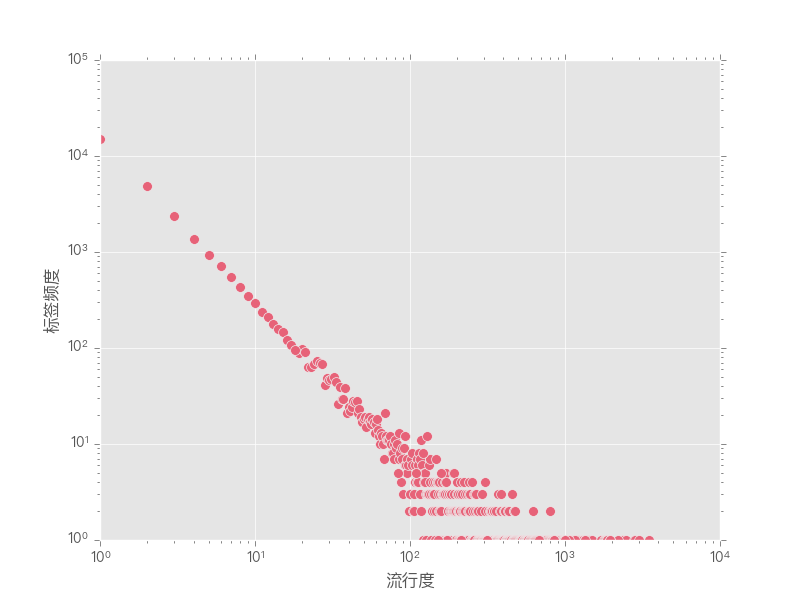
\includegraphics[width=0.48\linewidth]{images/powerlaw1.png}
}
\subfigure[LibraryThings]{
\label{fig:powerlaw:librarythings}
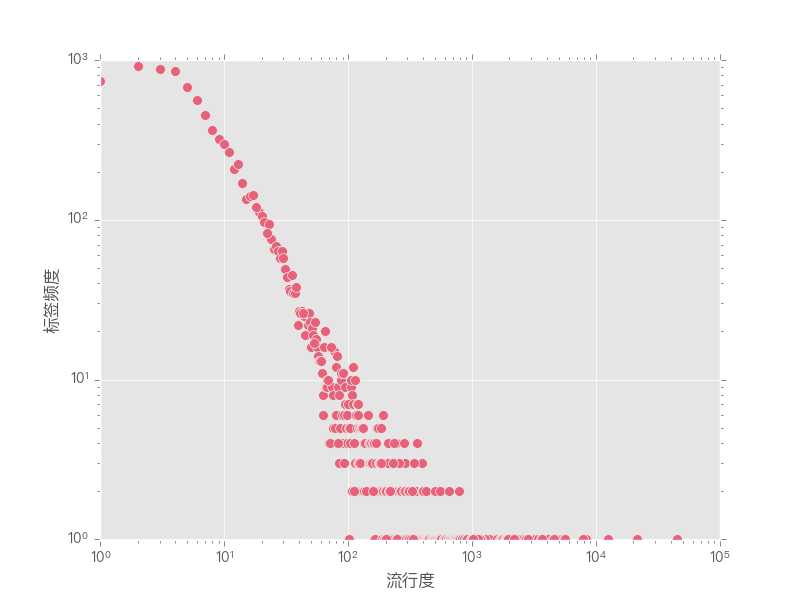
\includegraphics[width=0.48\linewidth]{images/powerlaw2.png}
}
\caption{标签流行度的长尾分布。横坐标是流行度 $k$ ,纵坐标是数据集中流行度为 $k$ 的标签总数 $n(k)$ 。}
\label{fig:powerlaw}
\end{figure}
从图中看出,大部分标签出现的频率都很低,只有很少的标签被经常使用。所以我们只考虑那些对评分预测具有帮助的标签,减小不相关标签引入的噪声。为了评估一个标签与评分是否相关,需要比较在该标签出现和不出现两种情况下的评分样本分布。我们使用 Wilcoxon 秩和检验,设置 $95\%$ 置信度,因此,当具有某个标签的评分与不具有该标签的评分之间具有显著差异时,我们认为该标签与评分是相关的。

\subsection{结合物品标签的协同过滤}
为了解决 UserItemTags 模型在预测时需要目标标签的限制,我们考虑任何用户赋予目标物品的全部相关标签集合 $TR(i)$ ,因为物品被赋予的任何相关标签都可能影响该物品的评分。如果一个标签被多次赋予一个物品,那我们认为这个标签更好的反映了该物品的特性,因此在模型中引入标签的出现频率,提升高频标签对评分的影响。我们用 $TRo_i$ 表示物品 $i$ 的全部相关标签数目(计入重复出现的标签),用 $TRo_i(t)$ 表示标签 $t$ 在物品 $i$ 上出现的次数。首先提出结合物品标签的协同过滤模型(collaborative filtering with item tags, 简称 ITCF),将物品标签信息融入预测模型中,对于给定用户 $u$ 和物品 $i$ ,按如下方式预测评分:
\begin{equation}
\hat{r_{ui}} =  \mu + b_i + b_u  +  p_u^T \cdot (q_i + \frac{1}{|TRo_i|}  \sum\limits_{t  \in TR(i)} {TRo_i(t) y_t}  ),
\end{equation}
其中,$p_u$,$q_i$ 和 $y_t$ 分别是用户 $u$、物品 $i$ 和标签 $t$ 的潜在特征向量。$\mu$ 是全部评分的平均值, $b_u$ 和 $b_i$ 是在用户 $u$ 和物品 $i$ 的偏移量(为了简明的描述我们的模型,之后的公式中不再显示地写出偏移项,而默认都是存在偏移项的)。模型参数的学习方法与传统的矩阵分解模型相同,采用随机梯度下降最小化正则平方误差:
\begin{equation}
\min_{q^*, p^*} {
\sum\limits_{u,i} {(r_{u,i} -  p_u \cdot (q_i + \frac{1}{|TRo_i|}\sum\limits_{t \in TR(i)}{TRo_i(t) y_t}))^2}
+ \lambda( \sum\limits_{u} ||p_u||^2+ \sum\limits_{i} ||q_i||^2 + \sum\limits_{t} ||y_t||^2 )}.
\end{equation}


遍历所有已知评分项(U-I-T-R),参数迭代方式如下:
\begin{equation}
\begin{aligned}
&-q_i \leftarrow q_i + \gamma \cdot(e_{ui} \cdot p_u -\lambda \cdot q_i)     \\
&-p_u \leftarrow p_u + \gamma \cdot(e_{ui} \cdot (q_i + \frac{1}{|TRo_i|}  \sum\limits_{t  \in TR(i)} {TRo_i(t) y_t})- \lambda \cdot p_u)    \\
&-\forall t \in TR(i) : y_t \leftarrow y_t + \gamma \cdot(e_{ui} \cdot p_u \cdot \frac{1}{|TRo_i|} \cdot TRo_i(t)  -\lambda \cdot y_t)     \\
\end{aligned}
\end{equation}

需要注意的是,在遍历已知项进行参数迭代时,对于每一个评分项都要对该物品所有的标签进行遍历。实际的数据集中,物品被标注的标签数目往往是巨大的,因此考虑到计算的时间复杂性,该模型是不那么可行的。

\subsection{标签主题聚类}

上面的模型中,我们将标签表示为低维的特征向量的形式,使物品标签信息融入了矩阵分解模型,然而该模型的问题是计算复杂度比较大。因此,我们对物品所关联的标签集 $TR(i)$ 进行聚类,去除冗余信息的同时扩充标签的含义,例如,“个性化”和“协同过滤”含义相似,可以将它们划分为同一类别考虑。将每个物品被赋予的标签集合看作“文档”,所有物品的标签集组成了文档集。由于标签是无序的,我们使用 LDA 主题模型进行文档分类, LDA 是典型的词袋模型,它不考虑文法以及词的顺序。

不同于其他聚类模型限定一篇文档只能属于一个类别,LDA 展示了文档在多个主题上表现出的相关性。LDA 从大量文档集合中发现一组主题 $\beta_{1:K}$,其中主题是关于词项的分布,这些主题通常是直观的可解释的。同时得到每篇文档的主题分布 $\theta_{1:J}$ ,将物品的标签集 $TR(i)$ 在 $K$ 个主题上的情况刻画出来,提供了物品标签集 $TR(i)$ 的低维表示。主题的词分布和文档的主题分布都是多项式分布。

为了结合协同过滤和主题模型,将物品的标签主题分布向量 $\theta_i$ 与之前矩阵分解中的物品特征向量 $q_i$ 结合起来,以它们的和作为物品的特征,从而评分预测为:
\begin{equation}
\hat{r_{ui}} =  p_u \cdot (q_i + \theta_i).
\end{equation}
因此,一个物品的标签主题分布揭示了该物品的特性,而一个用户特征向量每个维度上的数值表示了该用户对每个主题的偏好程度,这使得潜在特征向量是可解释的。在该模型中,标签主题的数目 $K$ 被限制与潜在特征的因子数相同,通常情况下,特征向量的维数 $f$ 在 20 到 200 之间\cite{Koren2009Matrix}。为了能更灵活地调整标签的主题分布情况,我们改变该模型的形式,为每个主题 $j$ 定义 $f$ 维特征向量 $z_j$ ,$Z \in R^{f*K}$ 表示主题的特征矩阵。将物品特征向量 $q_i$ 与加权平均的主题特征向量的和作为物品的特征表示,提出结合标签主题的协同过滤模型(collaborative filtering with tags topic,简称 TTCF),该模型以如下方式预测评分:
\begin{equation}
\label{TTCF}
\hat{r_{ui}} =   p_u^T \cdot (q_i +   \sum\limits_{j =1}^K {  {\theta_i}_j   z_j}  ),
\end{equation}
其中,主题特征的权值 ${\theta_i}_j $ 是主题分布 $\theta_i$ 在主题 $\beta_j$ 上的概率值,因为主题分布 $\theta_j$ 是多项式分布,所以权值的加和为 1,省去了计算加权平均时的分母部分。通过随机梯度下降最小化正则均方误差来学习模型的参数:
\begin{equation}
\begin{aligned}
&-q_i \leftarrow q_i + \gamma \cdot(e_{ui} \cdot p_u -\lambda \cdot q_i)     \\
&-p_u \leftarrow p_u + \gamma \cdot(e_{ui} \cdot (q_i +  \sum\limits_{j =1}^K {  {\theta_i}_j   z_j}  )- \lambda \cdot p_u)    \\
&-Z \leftarrow Z + \gamma \cdot(e_{ui} \cdot p_u \cdot  \theta_i^T -\lambda \cdot Z)     \\
\end{aligned}
\end{equation}

我们利用主题建模去除了标签的冗余,使得模型在计算复杂性方面变得可行,同时,主题建模对标签的含义进行了扩充,缓解了数据稀疏性问题。一个直观的好处是对于新物品的冷启动问题,可以从它的少量标签快速地获得主题,从而利用主题分布进行预测。


\section{跨域推荐模型}
在 3.2 中我们阐述了在单一域将标签信息引入矩阵分解的方法,利用主题建模缓解了数据稀疏性问题和冷启动问题。在本节中,我们引入跨域推荐的思想,将结合标签主题的协同过滤方法扩展到多个域上,利用辅助域的信息缓解目标域的数据稀疏性问题。

跨域推荐的关键挑战是在不同域的项目和用户之间发现有用的联系,通常所考虑的域之间看上去是不相关的,例如,音乐与感兴趣的地方,很难找到它们之间的关联。我们将标签作为连接不同域的桥梁,依赖于不同域中的重叠的标签词汇,例如,标签“romantic”可以用于描述一个电影,也可以是一首歌曲或是一处风景,换句话说,我们推测标签的影响是跨域的。因此,目标域可以学习到辅助域中的某个标签对评分的影响,即,如果在辅助域中的某个标签存在时,关联的评分通常较高,则可以将这种依赖关系从辅助域传递到目标域。将上面的预测模型$\eqref{TTCF}$ 扩展到多个域,对于每一个域 $d$ ,该推荐域中的评分预测模型为:
\begin{equation}
\hat{{r_d}_{ui}} = {p_d}_u^T \cdot ({q_d}_i +   \sum\limits_{j =1}^K {  {{\theta_d}_i}_j   z_j}  ),
\end{equation}
其中,${p_d}_u$ 和 ${q_d}_i$ 分别是推荐域 $d$ 所属的的用户和物品的潜在特征向量,${\theta_d}_i$ 是推荐域 $d$ 中的物品 $i$ 的标签主题分布。而主题的特征矩阵 $Z$ 则在多个域间共享,这样就通过标签主题在多个域间实现了相互影响。在参数学习中遍历两个域的可见项,利用随机梯度下降最小化正则均方误差。

\section{本章小结}
本章中,我们首先对基于标签的推荐问题进行了定义,然后提出了单个域上结合物品标签的协同过滤模型 ITCF,并指出了该模型在时间复杂性上的缺陷。继而提出结合标签主题的模型 TTCF,利用主题建模去除标签的冗余,并对标签的含义进行扩充,缓解了单个域上的物品冷启动问题和数据稀疏性问题。最后我们引入跨域推荐的思想,将单个域的模型扩展到多个域上,使得多个域的标签信息可以同时被利用来促进各个域上的预测效果。



    \cleardoublepage
    %!TEX root = ../main.tex
\chapter{实验与分析}
在本章中,我们介绍了在两个真实的数据集上进行的实验。为了评估提出模型的评分预测效果,我们从两个方面进行实验,首先测试该模型在单个域上的预测准确性相比传统方法的提升,然后在跨域的场景下评估该模型预测的质量,并与之前单个域上的结果进行比较,说明我们提出的模型是否利用跨域的标签信息缓解了数据稀疏性问题。

\section{数据集及预处理}
在我们的实验中使用了两个免费的真实数据集:包含 $200$ 万个评分的 MovieLens\footnote{MovieLens dataset: https://grouplens.org/datasets/movielens/20m/}  数据集,以及包含 70 万个评分的 LibraryThings\footnote{LibraryThing dataset: http://www.librarything.com/}数据集,这两个数据集的评分都在 1 到 5 范围内,步长为 0.5。MovieLens 包含 72,000 个用户对 10,000 个电影标注的 100,000 个标签,LibraryThings 包含 7,000 个用户对 37,000 个书籍标注的 200 万个标签。


MovieLens 数据集中的很多评分都没有关联的标签,在没有标签的情况下,我们的模型与传统的矩阵分解方法没有区别。既然我们的目的是通过实验验证引入标签信息是否对预测评分有好处,因此我们只考虑那些至少包含一个标签的评分。为了在跨域情况下减少不必要的干扰,我们使两个数据集的评分数相同,各自截取它们的前 1,0000 个具有标签的评分。在这两个评分的子集中,数据稀疏性都超过了 $99.5\%$ , MovieLens 中的标签覆盖了 LibraryThings 中 $25.31\%$ 的标签,而 LibraryThings 中的标签覆盖了 MovieLens 中 $15.09\%$ 的标签。LibraryThings 中不同的标签数更少,但是总共的标签数却更多,我们推测这些差异可以用于解释辅助域对于目标域的评分预测影响的大小。表\ref{dataset_feature}是数据集的详细统计信息。

\begin{table}[htbp]
\centering
\caption{MovieLens 和 LibraryThings 数据集的统计信息。}
\label{dataset_feature}
\begin{tabular}{|l|c|c|}
\hline
\rowcolor[HTML]{EFEFEF} 
           & MovieLens & LibraryThing \\ \hline
评分总数       & 10000     & 10000        \\ \hline
用户数        & 540       & 530          \\ \hline
物品数        & 3944      & 6092         \\ \hline
标签数        & 7284      & 4343         \\ \hline
全部标签       & 33875     & 44259        \\ \hline
每个用户的平均评分数 & 18.52     & 18.87        \\ \hline
每个评分的平均标签数 & 3.39      & 4.43         \\ \hline
标签覆盖率      & 15.09\%   & 25.31\%      \\ \hline
数据稀疏度      & 99.53\%   & 99.69\%      \\ \hline
\end{tabular}
\end{table}

\section{实验设计}
我们设计两组实验:第一组实验测试提出的模型在单个域上的预测准确性,并与其他模型进行比较分析;另一组实验在跨域的场景下进行,对比跨域模型和之前单个域上模型的效果。
\subsection{数据集划分}
为了保证实验结果的准确性,我们采用交叉验证过程。首先将数据集的评分数据均分成五个部分,我们使用其中的一份数据作为测试集,而剩余的部分作为训练集。将这个过程重复五次,使得我们可以利用五个不同的测试集来测试模型的效果。

为了验证模型在不同数据稀疏程度下的表现,我们将选中的训练集再均分为十份,因此,为了验证在数据非常稀疏的情况下模型的表现,我们使用 $10\%$的训练数据进行实验,之后每次加入一份数据,以模拟实际系统中数据不断丰富的情况。

在跨域的场景下,目标域数据集的划分方式与上面所述相同,对于辅助域则将全部的数据划分为训练集。

\subsection{评价标准}
准确度是度量一个推荐系统预测能力的指标,通常将预测的行为与测试集上行为的重合度作为预测准确度。推荐的任务可以分为 TopN 推荐和评分预测两种:网站提供推荐服务时一般会给用户一个猜你喜欢列表,这种推荐叫做 TopN 推荐,TopN 推荐的准确度一般利用召回率(Recall)和精确率(Precision)来度量;而有些网站具有用户给物品打分的功能,评分预测就是预测用户给他未评分的物品的评分,通常用平均绝对误差(MAE)和均方根误差(RMSE)来评估预测准确度。本文使用的数据集是五分制的评分形式,因此我们的实验属于评分预测的范畴。

对于测试集中的一个用户 $u$ 和物品 $i$ ,另 $r_{ui}$ 是用户 $u$ 对物品  $i$  的实际评分,而 $\hat{r_{ui}}$  是推荐算法给出的预测评分,那么 MAE 定义为:
\begin{equation}
MAE = \dfrac   {\sum\limits_{u,i \in T}  |r_{u,i} - \hat{r_{ui}}| } {|T|}.
\end{equation}
RMSE 采用均方根的形式计算预测误差,它的定义为:
\begin{equation}
RMSE = \sqrt{  \dfrac   {\sum\limits_{u,i \in T}  (r_{u,i} - \hat{r_{ui}}) ^2 } {|T|}   }.
\end{equation}
相比于 MAE,RMSE 的评价标准更加严格,它在防止过拟合方面更加灵敏,所以我们在进行模型参数训练时采用 RMSE 来衡量模型推荐效果。

我们将提出的模型与两个之前提到的 SVD 和 UserItemTags 模型进行对比,其中 SVD 模型无法利用辅助域的额外信息,因为两个域的用户和物品是没有交集的。在进行不同模型的对照实验时,为了全面地评估模型的性能,我们也比较了不同模型的 MAE 的大小。

\subsection{参数设置}
我们通过实验分析不同参数组合对模型的影响,在实验数据集上将模型调整到最优状态。

$f$ 作为潜在特征向量维度,对模型的推荐效果和运算效率至关重要,当 $f$ 值比较小时,时间复杂度会比较低,但是可能会损失预测的准确度,因此我们需要在两者之间找到一个折中的 $f$ 值。首先根据经验固定其他参数,对不同的 $f$ 取值进行实验,确定之后实验中 $f$ 的值。
\begin{figure}[htbp]
\centering
\subfigure[MovieLens]{
\label{fig:nfactors:movielens}
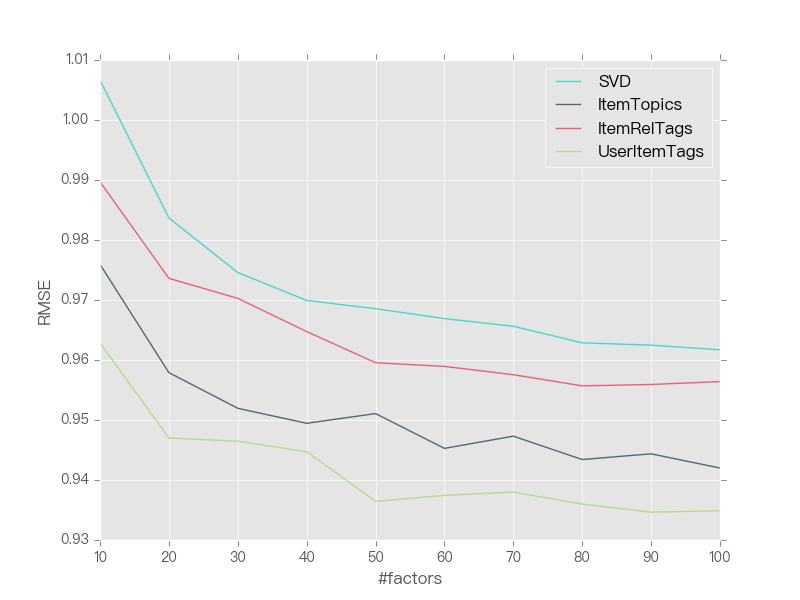
\includegraphics[width=0.48\linewidth]{images/factors1.png}
}
\subfigure[LibraryThings]{
\label{fig:nfactors:librarythings}
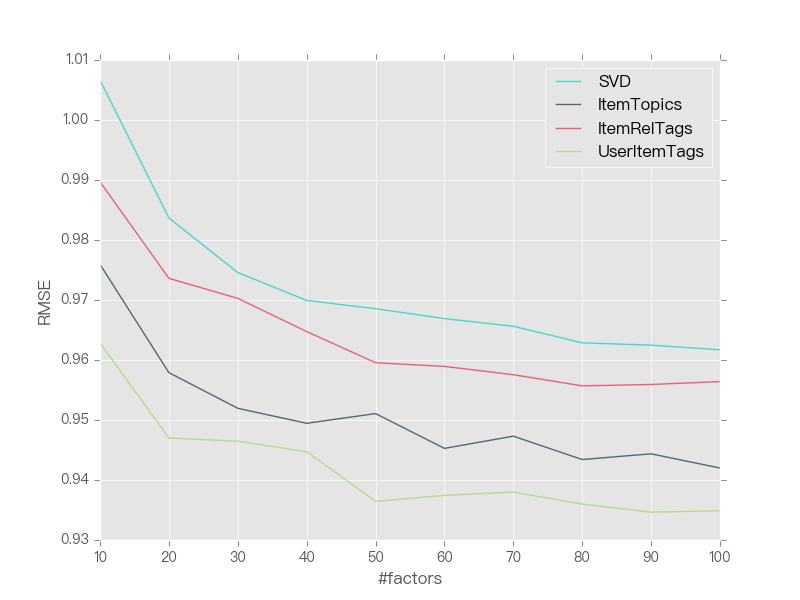
\includegraphics[width=0.48\linewidth]{images/factors1.png}
}
\caption{特征向量维度 $f$ 对模型 RMSE 的影响。}
\label{fig:nfactors}
\end{figure}
图 \ref{fig:nfactors} 显示了 $f$ 在 10-100 之间取值时不同模型的预测效果,可以看到随着 $f$ 的增大,各模型的准确度呈上升的趋势,并逐渐趋于稳定。处于对计算复杂性的考虑,我们在之后实验中将 $f$ 设置为 100。

固定参数 $f$ 之后,我们利用网格搜索的方式获得其它参数的最优值,各模型在两个数据集上的最优参数见表 \ref{params}。

\begin{table}[htbp]
\centering
\caption{模型的最优参数。}
\label{params}
\begin{tabular}{|l|c|c|c|c|}
\hline
             & \multicolumn{2}{c|}{MovieLens} & \multicolumn{2}{c|}{LibraryThings} \\ \hline
             & $\gamma$      & $\lambda$      & $\gamma$        & $\lambda$        \\ \hline
SVD          & 0.01          & 0.04           & 0.01            & 0.02             \\ \hline
UserItemTags & 0.01          & 0.04           & 0.01            & 0.01             \\ \hline
ITCF         & 0.01          & 0.02           & 0.01            & 0.02             \\ \hline
TTCF         & 0.005         & 0.002          & 0.04            & 0.01             \\ \hline
\end{tabular}
\end{table}

\subsection{LDA 主题建模}
本文采用开源的 Python 程序包 lda\footnote{http://pythonhosted.org/lda/} 进行标签主题建模,它以吉布斯采样的方式实现了隐式狄利克雷分布(LDA)。我们在实验中设置 lda 的参数 $\alpha=0.1​$ 、$\eta = 0.01​$ ,迭代次数为 2000。为了观察提取主题的有效性,我们设置主题数 $K=20$ ,表\ref{Topics}是通过训练 LDA 模型得到的两个数据集上的 Top 词表。

我们发现属于相同主题的标签项具有相近的意思,即利用主题建模完成了标签聚类。因此,根据每个主题对应的词表可以很容易解释主题的含义,我们将凭经验总结的主题词列在了每个主题的上面。

\begin{table}[htbp]
\footnotesize
\centering
\caption{从两个数据集学习到的主题。}
\label{Topics}
\begin{tabular}[c]{ccccccc}
\hline
\hline
\multicolumn{7}{c}{MovieLens 的主题}                                                             \\
喜剧        & 间谍         & 冒险           & 黑色幽默        & 犯罪       & 科幻        & 战争           \\ \hline
comedy    & politics   & fantasy      & dark comedy & quentin  & sci-fi    & true story   \\ 
funny     & espionage  & adventure    & quirky      & violence & dystopia  & world war ii \\ 
animation & religion   & johnny depp  & satire      & action   & aliens    & classic      \\ 
pixar     & action     & magic        & drugs       & crime    & space     & war          \\ 
disney    & tom cruise & stylized     & cult        & revenge  & robots    & history      \\ 
parody    & thriller   & martial arts & witty       & drugs    & future    & tom hanks    \\ 
christmas & conspiracy & surreal      & satirical   & violent  & adventure & racism       \\ 
hilarious & corruption & fairy tale   & zombies     & mafia    & cyberpunk & prison       \\ \hline
% \noalign{\bigskip}  
\hline
\hline
\multicolumn{7}{c}{LibraryThings 的主题}                                                             \\ 
魔幻        & 历史         & 幽默           & 经典        & 传记       & 科幻        & 惊悚           \\ \hline
fantasy    & history   & humor      & classic & nonfiction  & sci-fi    & mystery   \\ 
magic     & religion  & humour    & literature      & memoir & novel  & crime \\ 
discworld & philosophy   & comics  & poetry      & history   & dystopia    & thriller      \\ 
mythology     & war     & satire        & manga       & biography    & space     & suspense          \\ 
wizards    & christianity & comedy     & british        & reference  & aliens    & murder      \\ 
novel    & nonfiction   & funny & drama       & travel    & fantasy    & detective    \\ 
dragons & biography & surreal      & romance   & autobiography  & time travel & adventure       \\ 
adventure & politics & art   & england     & essays    & fiction & novel       \\ \hline
\hline
\end{tabular}
\end{table}

\section{实验结果分析}
本节中,我们按照实验设计中的方法得到模型的参数,并对模型进行训练。通过对比不同模型间的推荐准确性 RMSE,分析各模型的优劣。第一组实验测试在单个域上的预测准确性,第二组是在跨域的场景下实验,并将得到的结果与之前单个域进行对比。

\subsection{单个域推荐}
为了验证本文提出的两个模型的预测效果,我们将它们与两个优秀的推荐算法进行比较:SVD 模型,即基于矩阵分解的协同过滤算法;UserItemTags 模型,在 SVD 中结合了目标用户对目标物品的标签信息。我们从 RMSE 和 MAE 两个角度分别在 MovieLens 和 LibraryThings 数据集上衡量各模型的性能,并将实验结果数据用柱状图展示出来,如图 \ref{fig:bar} 所示,其中数值越低表示模型的推荐准确度越高。
\begin{figure}[!htbp]
\centering
\subfigure[RMSE]{
\label{fig:bar:rmse}
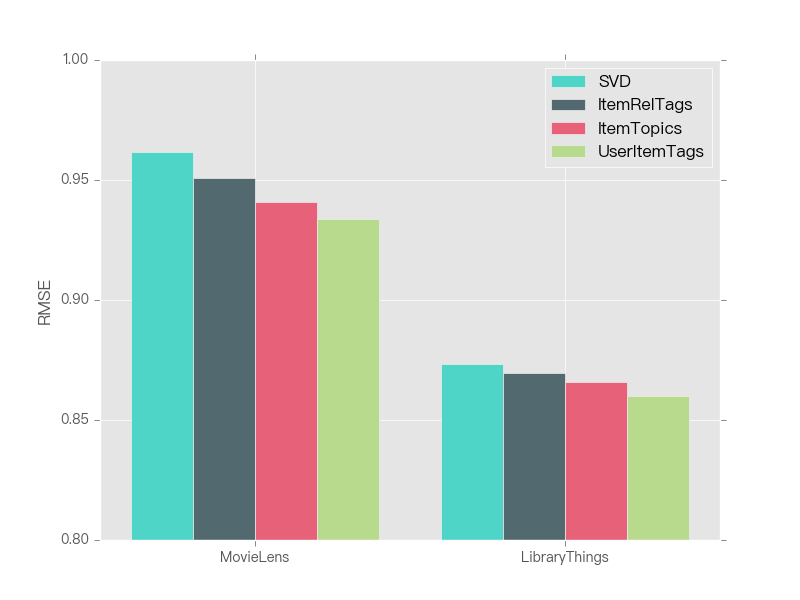
\includegraphics[width=0.48\linewidth]{images/bar_rmse.png}
}
\subfigure[MAE]{
\label{fig:bar:mae}
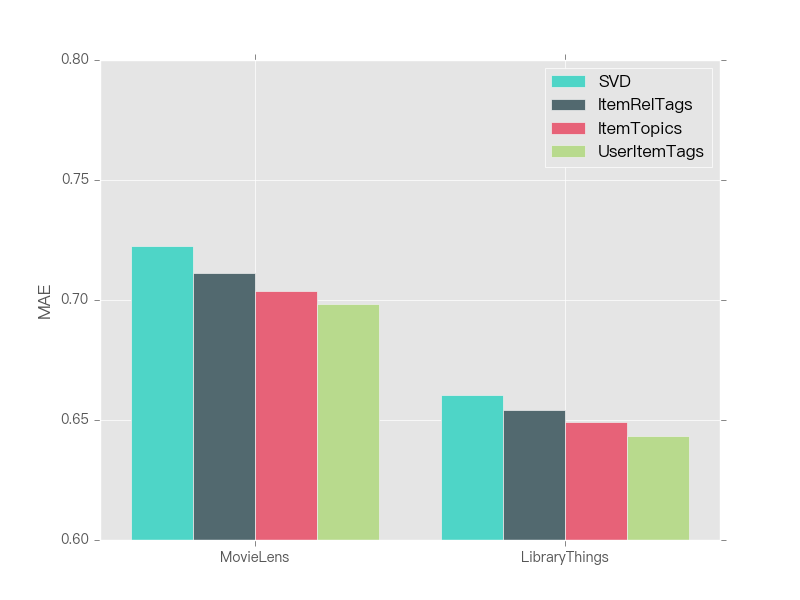
\includegraphics[width=0.48\linewidth]{images/bar_mae.png}
}
\caption{不同模型的推荐准确度对比。}
\label{fig:bar}
\end{figure}

从结果中看出,我们提出的两个模型 ITCF 和 TTCF 在预测准确性上都优于传统的 SVD 矩阵分解算法,由此证明了引入额外的标签信息对于预测效果的提升是有帮助的。因为 UserItemTags 模型必需目标用户对目标物品的标签,因此在推荐准确性上强于我们的模型,但是我们的模型解除了这项限制,具有更广泛的适用性。对于我们提出的两个模型,它们都利用了物品的标签信息,相比于 ITCF 模型,TTCF 利用主题建模对标签进行了聚类,去除了冗余信息的同时扩充了标签的含义,使得模型的推荐效果有了显著提升。
\begin{figure}[!htbp]
\centering
\subfigure[MovieLens]{
\label{fig:single_plot:MovieLens}
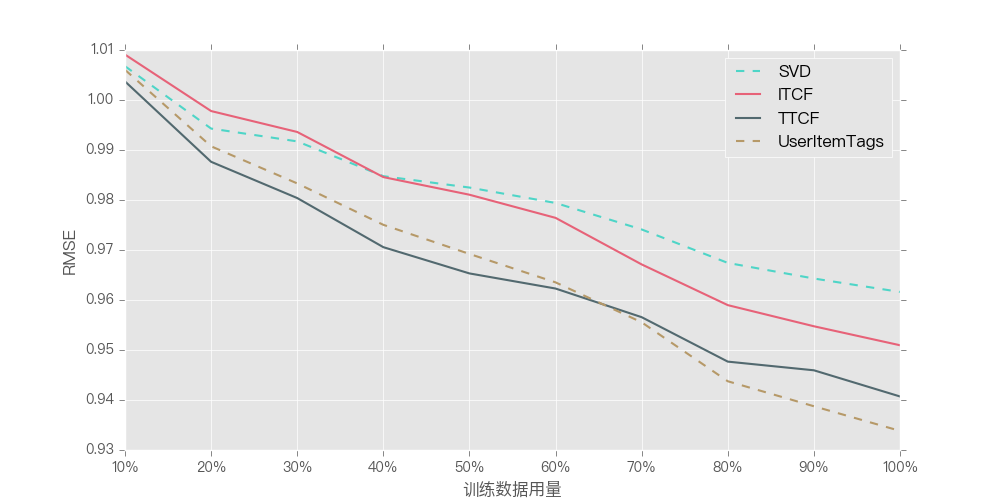
\includegraphics[width=\linewidth]{images/plot1.png}
}
\subfigure[LibraryThings]{
\label{fig:single_plot:LibraryThings}
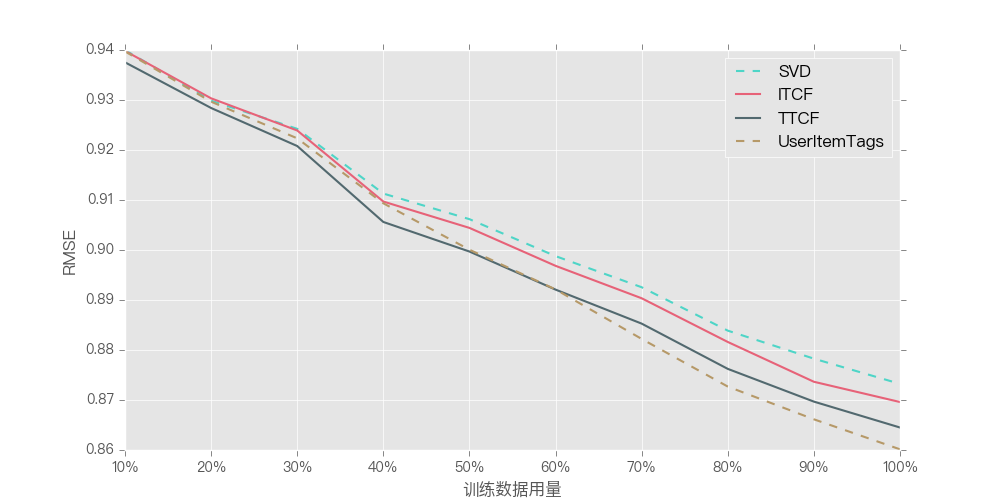
\includegraphics[width=\linewidth]{images/plot2.png}
}
\caption{不同数据用量下模型的 RMSE 对比。}
\label{fig:single_plot}
\end{figure}

接下来我们得到了在不同数据稀疏程度下各个模型的实验结果,图 \ref{fig:single_plot} 展示了不同模型的 RMSE 在各个数据用量上的数值.可以看出,在数据用量比较多的情况下,模型的预测准确度与上面得到的结果相同,但是在数据比较稀疏时,各模型表现出的性能有些不同。由于 TTCF 模型利用聚类扩充了标签含义,使得它仅利用少量标签即可获得很好的预测效果,因此在数据用量比较小时该模型的准确性超过了 UserItemTags 模型的准确性,可以说 TTCF 模型很好地缓解了数据稀疏性问题。另外,我们看到在 MovieLens 数据集上,当数据用量小于 $40\%$ 的情况下,ITCF 模型的预测准确性甚至低于 SVD 模型,我们推测这是因为当物品的标签很少时,少量的标签不能准确地描述物品的性质,甚至对评分预测产生了误导,而随着可利用的物品标签的丰富,预测准确性也逐渐超过了 SVD 模型。


\subsection{跨域推荐}
接下来我们在两个跨域的场景下验证提出的 Cross-TTCF 模型,第一种情况将 MovieLens 作为目标域,LibraryThings 作为辅助域,第二种情况将 LibraryThings 作为目标域,而 MovieLens 作为辅助域。同样,为了验证不同数据稀疏程度下模型的性能,我们使用不同的数据用量进行实验,并将得到的结果与单个域的模型进行对比。

图 \ref{fig:cross_plot}展示了不同数据用量下模型的预测准确度,可以看出,相比于只使用单个域的数据,跨域模型利用辅助域的评分和标签信息从整体上提升了目标域的推荐性能。
然而,在 LibraryThings 作为目标域的情况下,我们看到当数据用量很少时(少于 20\%),辅助域的标签信息并不能帮助提升预测的准确性。我们认为这是因为辅助域(MovieLens)中的标签覆盖了相对更多的目标域(LibraryThings)中的标签,因此当目标域只使用 10\% 的数据时,辅助域中标签和评分的关系会对预测模型造成很大的影响。换句话说,模型利用标签预测了辅助域中的评分,而不是目标域的评分。
\begin{figure}[!h]
\centering
\subfigure[MovieLens 作为目标域,LibraryThings 作为辅助域]{
\label{fig:cross_plot:MovieLens}
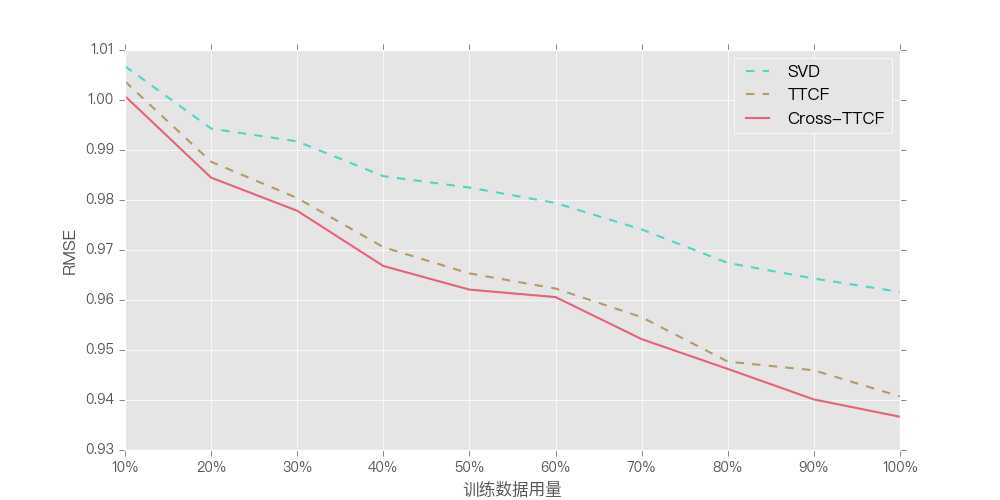
\includegraphics[width=\linewidth]{images/cross1.png}
}
\subfigure[LibraryThings 作为目标域,MovieLens 作为辅助域]{
\label{fig:cross_plot:LibraryThings}
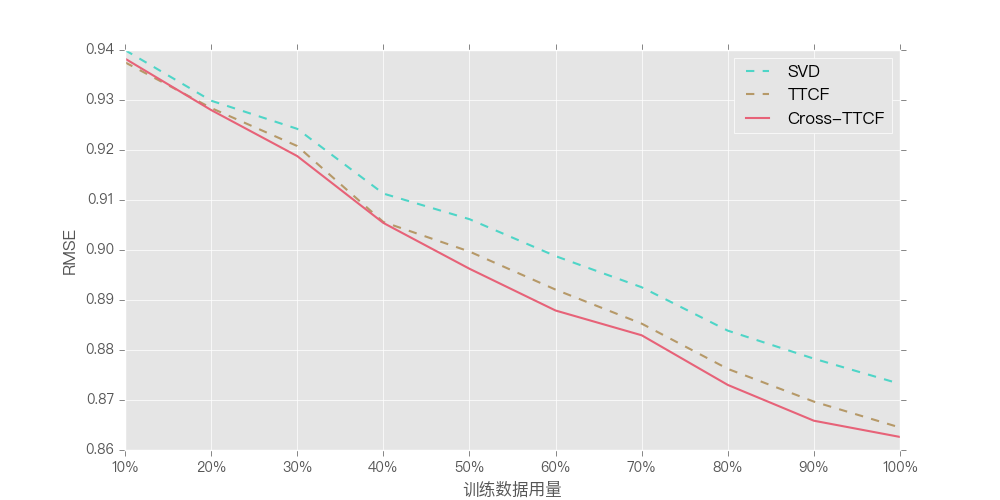
\includegraphics[width=\linewidth]{images/cross2.png}
}
\caption{单个域和跨域模型的 RMSE 对比。}
\label{fig:cross_plot}
\end{figure}

\section{本章小结}
本章中,我们首先对实验数据集进行了预处理,并得到了数据集的统计信息。之后我们阐述了实验的设计方案,采用 5 折交叉验证评估模型的预测准确性,利用网格搜索获取模型的最优参数,并解释了标签主题的意义。我们从两个方面进行对比实验并得出结论:在单个域上,我们提出的 TTCF 模型相比于传统矩阵分解模型具有明显优势,并且在数据比较稀疏的情况下,TTCF 模型的预测性能超过了 UserItemTags 模型,说明结合标签主题的模型对于缓解数据稀疏性问题具有良好的效果;在跨域的场景下,通过与单个域模型的对比,证明了我们的模型利用辅助域的标签和评分信息提升了目标域的推荐准确性,并讨论了跨域推荐中存在的问题。



    \cleardoublepage
    %!TEX root = ../main.tex
\chapter{总结和展望}

\section{本文工作总结}
在本文中,我们首先梳理了推荐算法的研究现状,并介绍了推荐系统中的数据稀疏和冷启动问题。为了缓解这两个问题,我们提出了一个结合标签主题的跨域推荐模型,在这个模型中,我们使用主题建模采集物品标签中的语义信息,并将语义信息引入了基于矩阵分解的协同过滤模型,然后以标签主题作为跨域传递的信息,将模型扩展到跨域的场景。最后通过对 MovieLens 和 LibraryThing 数据集进行的一系列实验,证明了该模型可以利用额外的标签信息缓解数据稀疏和冷启动问题,并且可以在没有共享用户的情况下,利用辅助域的评分和标签信息提升目标域的评分预测效果。
本文工作总结如下:
\begin{enumerate}
\item 对推荐系统的背景和研究现状进行了介绍,并阐述了目前研究中所面临的困难与挑战。
\item 对本文的相关研究成果进行了综述,详细阐述了经典的协同过滤模型,以及主题建模和跨域推荐的思想。
\item 将标签信息结合到传统的矩阵分解模型,并利用主题建模采集了标签的语义信息,使得模型可以很好地处理数据稀疏和冷启动问题,之后将模型扩展到多个域上,利用辅助域的标签和评分信息提升了目标域的评分预测效果。
\item 阐述了模型参数的设置方法,在两个真实的数据集上对模型进行了评估,并与其它的模型进行了对比实验。
\end{enumerate}

\section{未来工作展望}
本文将主题建模和跨域推荐的思想结合到传统的矩阵分解模型中,充分利用标签这种隐式反馈信息缓解了数据稀疏和冷启动问题,从而获得了更好的推荐效果。同时,有几个方面值得未来的继续探索:
\begin{enumerate}
\item 本文使用 LDA 主题建模的方式对标签进行聚类,去除冗余信息提升了算法效率,并且扩充了标签的含义,提升了在数据稀疏情况下的预测效果。那么,我们可以尝试使用其它的标签聚类方法,例如比较流行的基于标签共现的标签聚类算法\cite{王娅丹2015标签共现的标签聚类算法研究},并对比采用不同聚类算法时模型的预测效果。
\item 我们认为物品的标签集合反应了物品的特征,因此提出的模型主要针对物品的标签集进行信息挖掘。另一方面,我们可以尝试挖掘用户标签集中的信息,因为用户通常具有某些方面的偏好,而这些偏好会反应在用户标注的标签上。
\item 本文提出的模型可以适应多个域的情况,只要这些域中有重叠的标签集合。
因此可以尝试在多个数据集上对模型进行测试,以充分利用不同域之间的关联性。
\end{enumerate}


    \cleardoublepage
    \renewcommand{\thechapter}{}
    \bibliographystyle{data/gbt7714-2005}
\bibliography{data/bibliography}
\addcontentsline{toc}{chapter}{\bibname}

    \cleardoublepage
    \chapter*{致谢}
\addcontentsline{toc}{chapter}{致谢}
\markright{致谢}

首先,我衷心感谢我的导师郑小林副教授在学习和生活中给予我的谆谆教诲和悉心关怀。本论文从选题、构思、修改到成文,每个环节都凝结了实验室老师大量的心血,充斥了 实验室学长学姐的耐心指导。郑小林教授专业知识渊博,治学态度严谨,在学术上精益求精、积极进取,在工作中求真务实,在生活中平易近人,给我留下了深刻的印象。在短短几个月 相处时间里,我深深感受到了郑老师出色的人格魅力,这在以后的求学道路上无疑给我树立 了旗帜鲜明的方向标,是我一生取之不尽的宝贵财富。

此外,我要感谢浙江大学电子服务研究中心的所有师兄师姐们,在学习和工作中离不开 他们的支持和帮助。

感谢计算机学院的各位老师,谢谢你们在我本科生阶段带领我进入丰富多彩的计算机 科学与技术的世界。

感谢对我本科论文进行评审的各位专家教授,感谢你们对论文的指导和提出的宝贵意见。

我要特别感谢我的父母,他们在我的成长中起到了不可磨灭的影响,是我人生中最重要的依靠和指引。

最后,感谢所有给予我指导、帮助、关心和支持的老师、亲人和朋友们。

\begin{flushright}
杨煜溟

2017 年 5 月
\end{flushright}


    \cleardoublepage
  }

  {
    \backmatter

    \pagestyle{empty}

    % {
  \setlength{\parindent}{0em}
  \linespread{1}

  \vspace*{-2.2em}

  {
    \centering
    \songti\erhao\bfseries
    本科生毕业论文(设计)任务书 \par
  }

  \vspace{2.1em}

  {
    \songti\xiaosi\bfseries
    一、 \; 题目 \; \underline{\makebox{\zjutitlec}}
  }


    \vspace{1.1em}

  {
    二、 \; 指导教师对毕业论文(设计)的进度安排及任务要求
  }

    
    该毕业论文要求在对协同过滤模型相关国内外研究现状进行深入分析的基础上, 重点围绕结合标签的跨域推荐模型展开研究。实验过程要严谨有效,实验结果要清晰可信。
    进度安排如下:
    3.01-3.15 研究方案确定 
    3.16-4.15 模型的建立与算法实现 
    4.15-5.15 实验与分析
    5.16-5.30 论文撰写

    \vspace{15.5em}

    \hfill 起讫日期 \hspace{2em} 年 \hspace{1em} 月 \hspace{1em} 日 \; 至 \hspace{2em} 年 \hspace{1em} 月 \hspace{1em} 日

    \vspace{1.3em}

    \hfill 指导教师(签名) \; \underline{\hspace{4em}} \; 职称 \; \underline{\hspace{4em}}

    \vspace{2.35em}

    三、 \; 学院审核意见

    \vspace{13.95em}

    \hfill 负责人(签名) \; \underline{\hspace{4em}}

    \vspace{1.3em}

    \hfill \hspace{2em} 年 \hspace{1em} 月 \hspace{1em} 日 \par
  }
}

    % {
  \setlength{\parindent}{0em}
  \linespread{1}

  \vspace*{-2.1em}

  {
    \centering
    \songti\xiaoer\bfseries
    毕~~业~~论~~文~~(设~~计)~~考~~核 \par
  }

  \vspace{1.1em}

  {
    \songti\sihao\bfseries
    一、\; 指导教师对毕业论文(设计)的评语 \par
  }

  跨域推荐是当前的研究热点,作者以该方向为研究目标,选题具有较高的应用价值。作者在对推荐算法的国内外研究现状进行深入分 析的基础上,提出了结合标签主题的跨域推荐方法。通过在 MovieLens 和 LibraryThings 数据集上开展的实验分析表明,该方法具有一定的先 进性和较高的实用性。论文工作表明作者具有扎实的基础理论知识, 以及一定的科研工作的能力。论文条理清楚,层次分明,达到了本科毕业论文的要求。

  \vspace{8em}

  {
    \songti\xiaosi\bfseries
    \hfill 指导教师(签名) \; \underline{\hspace{5em}}

    \vspace{0.1em}

    \hfill \hspace{2em} 年 \hspace{1em} 月 \hspace{1em} 日 \par
  }

  \vspace{0.7em}

  {
    \songti\sihao\bfseries
    二、 \; 答辩小组对毕业论文(设计)的答辩评语及总评成绩:
  }

  \vspace{14.7em}

  {
    \renewcommand{\arraystretch}{1.5}
    \songti\xiaosi\bfseries
    \hfill \begin{tabular}{|c|m{4.1em}|m{4.1em}|m{4.1em}|m{9.1em}|c|}
      \hline
      成绩比例 & {\centering 开题报告 \\ 占(20\%)} & {\centering 外文翻译 \\ 占(10\%)} & {\centering 文献综述 \\ 占(10\%) } & {\centering 毕业论文(设计) \\ 质量及答辩占(60\%)} & 总成绩 \\
      \hline
      分值 & & & & & \\
      \hline
    \end{tabular} \par
  }

  \vspace{2em}

  {
    \songti\xiaosi\bfseries
    \hfill 答辩小组负责人(签名) \; \underline{\hspace{5em}}

    \vspace{0.1em}

    \hfill \hspace{2em} 年 \hspace{1em} 月 \hspace{1em} 日 \par
  }
}

  }

\end{document}
